\documentclass{article}

\usepackage[utf8x]{inputenc}
\usepackage[spanish]{babel}
\usepackage[margin=3.5cm]{geometry}
\usepackage{amsmath}
\usepackage{amssymb}
\usepackage{graphicx}
\usepackage{algorithm}
\usepackage{algorithmic}

\usepackage{ stmaryrd }

\usepackage{ upgreek }

\usepackage{listings}

\linespread{1.2}

\usepackage{color}
\usepackage{listings}

\definecolor{javared}{rgb}{0.6,0,0} % for strings
\definecolor{javagreen}{rgb}{0.25,0.5,0.35} % comments
\definecolor{javapurple}{rgb}{0.5,0,0.35} % keywords
\definecolor{javadocblue}{rgb}{0.25,0.35,0.75} % javadoc
 
\lstset{language=Java,
basicstyle=\ttfamily,
keywordstyle=\color{javapurple}\bfseries,
stringstyle=\color{javared},
commentstyle=\color{javagreen},
morecomment=[s][\color{javadocblue}]{/**}{*/},
numbers=left,
numberstyle=\tiny\color{black},
stepnumber=1,
numbersep=10pt,
tabsize=4,
showspaces=false,
showstringspaces=false}

\title{ Computación Concurrente \\ \Large{Tarea 9}
\author{
  Diego Goméz Montesinos
  \and
  José Emiliano Cabrera Blancas
  }
\date{6 Mayo 2014}
}
\begin{document}
\maketitle
\begin{enumerate}
  
\item{
    \textsl{
      Los programadores de la compañía de computación Flaky diseñaron
      el protocolo que se muestra a continuación para lograr la
      exclusión mútua de n-hilos. Para cada pregunta, presenta una
      prueba o despliega una ejecución donde falle.
    }
      \begin{itemize}
        \item{\textsl{¿El protocolo satisface la exclusión mútua?}}
        \item{\textsl{¿Este protocolo es starvation-free?}}
        \item{\textsl{¿Este protocolo es deadlock-free?}}
      \end{itemize}

      \renewcommand{\lstlistingname}{}
\begin{lstlisting}[frame=single]
class Flaky implements Lock {
   private volatile int turn ;
   private volatile boolean busy = false ; 
   
   public void lock () {
      int me = ThreadID.get();
      do {
         do {
            turn = me;
         } while (busy);
         busy = true;
         } while (turn != me);
   }

   public void unlock () {
      busy = false;
   }
}
\end{lstlisting}
      
      Primero recordemos las definciones de lo que nos piden demostrar
      o dar una contradición.
      \begin{itemize}
      \item{\textbf{Exclusión Mutua:} Las secciones criticas entre
          los procesos nunca se van a translapar.}

        \item {\textbf{Starvation-free:} Cada hilo que intente
            adquirir el \textit{lock} eventualmente lo logra.}

        \item{\textbf{Deadlook-free:} Si algún hilo intenta conseguir
            el \textit{lock}, entonces ese mismo hilo u otro hilo
            obtendra el \textit{lock}.}
      \end{itemize}

      \begin{itemize}
        \item{\textbf{Exclusión Mutual}\\
            Podemos observar que si esta propiedad no se cumpliera,
            implicaria que existe al menos una ejecución en donde 2 o
            más procesos adquieren el \textit{lock} antes de que se
            liberen.\\

            Demostración (por contradicción):\\
            Supongamos que 2 o más procesos adquieren el \textit{lock}
            antes de que este se libere.\\

            Si dos o más procesos adquirieron el \textit{lock} eso
            quiere decir que en algún momento ellos procesaron 
            \textit{turn != me} como \textit{false} y por lo tanto
            tuvieron que procesar \textit{while(busy)} como
            \textit{false}.\\
            Pero para que eso pase, cada proceso que obtuvo el
            \textit{lock} ejecuto \textit{turn = me}, por lo que el
            último que lo escribio fue el único que vio \textit{turn
              != me} como \textit{false}, lo cual es una contradicción
            por que todos vieron \textit{turn != me} como
            \textit{false}, por lo tanto la exclusión mutua se cumple.\\
          }

        \item{\textbf{Starvation-free:} Afirmamos que esta propiedad
            no se cumple, lo cual quiere decir existe una ejecución
            donde al menos un hilo no logra obtener el \textit{lock}
            nunca.\\

            Ejecución:\\
            Tenemos un escenario donde el \textit{lock} esta libre.\\
            El proceso A comienza a ejecutar el código para pedir el
            \textit{lock}, y ejecuta la linea \textit{turn =
              me}, después algún otro proceso entra rápido y ejecuta
            todo el código del metodo \textit{lock}. El proceso A
            entra en el \textit{loop} hasta que \textit{busy} sea
            \textit{false}, se libéra el \textit{lock} y la última
            línea que A procesa es \textit{turn = me} y otra vez,
            algún otro proceso entra rápido a ejecutar el código del
            método \textit{lock} y A se queda en el \textit{loop}.\\
            Este caso lo podemos repetir de forma infinita, y
            claramente A nunca obtiene el \textit{lock} aunque sea el
            primer proceso que lo pidio.\\

          }

          \item{\textbf{Deadlook-free:} Afirmamos que esta propiedad
              no se cumple, lo cual quiere decir que existe una
              ejecución donde 2 o más procesos solicitan el
              \textit{lock}, este no esta siendo ocupado por otro hilo
              y aún así el recurso nunca se les es liberado.\\

              Ejecución:\\
              Tenemos un escenario donde el proceso A y B van a
              solicitar el \textit{lock} y ningún otro proceso lo esta
              ocupando.\\
              El proceso A comienza a ejecutar el código del método
              \textit{lock}, llega hasta la linea \textit{busy = true}
              y justo después el proceso B comienza a ejecutar el
              mismo método \textit{lock}, y la primera linea que
              ejecuta es \textit{turn = me}, ahora el proceso A
              continua con su ejecución y se encuentra con que
              \textit{turn != me}  es \textit{true}, por lo que
              regresa a ejecutar el inicio del \textit{loop}, como A
              escribio \textit{busy = true}, el proceso B y el proceso
              A se quedaran ejecutando el \textit{loop} de forma
              infinita  y de hecho
              cualquier otro proceso que entre obtendra el
              \textit{lock}.\\
            }
      \end{itemize}
    }

\item{
    \textsl{
      Durante la exposición se mostró la construcción de un sistema
      bounded-Timestamp para 2 y 3 hilos, con base en la explicación
      dada, construya uno para 4 hilos y responda adicionalmente las
      siguientes preguntas.
    }

    Siguiendo la forma recursiva de construir la gráfica que representa
    el sistema Bounded-Timestamp, la construcción de $T^{4}$ da como resultado:
    \begin{center}
       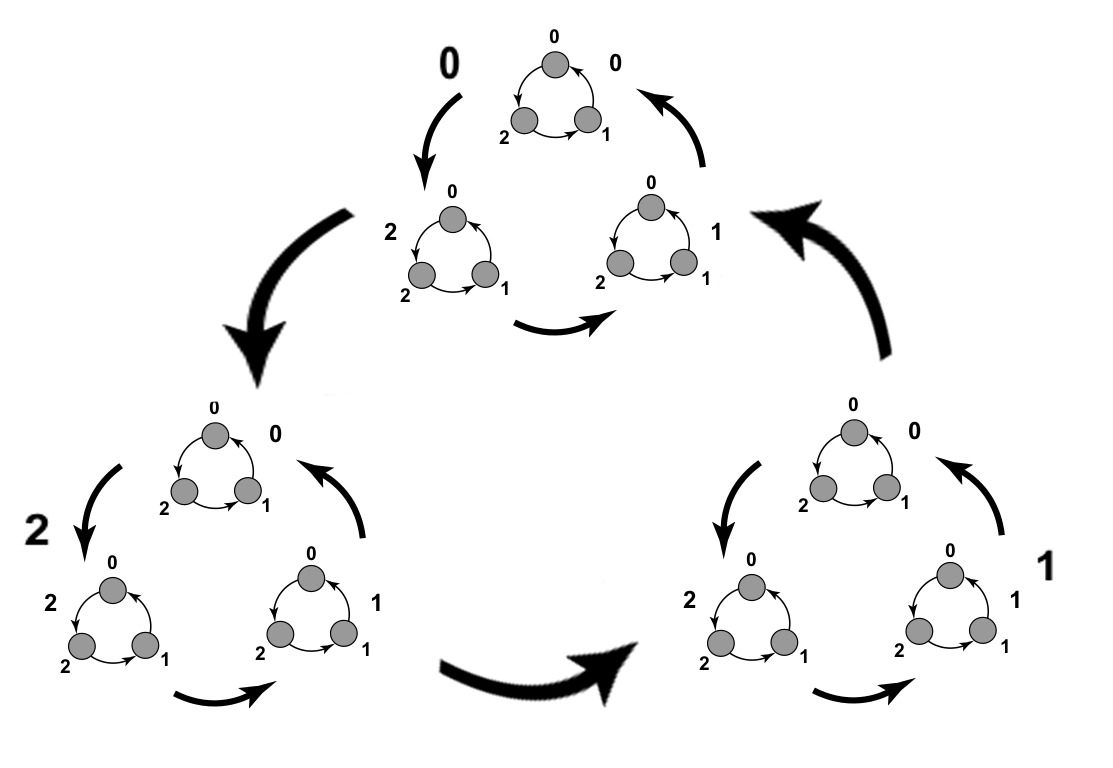
\includegraphics[scale=0.25]{t4.png}
    \end{center}

    \begin{itemize}
    \item{\textsl{
          En el sistema construido para 3 hilos puede observarse que
          existen más vértices que procesos y podría suponerse que es
          posible el utilizarlo para 4 hilos, muestre un ejemplo que
          contradiga esta suposición.
        }}

        Supongamos que tenemos 4 hilos: $A, B, C$ y $D$. $A$ está en
        $00$, $B$ en $01$, $C$ en $10$, y $D$ en $20$. Supongamos que
        $D$ se retrasa y $C$ termina y quiere de nuevo entrar,
        entonces tendría que acomodarse en un lugar tal que domine
        a $A, B$ y $D$, y ese lugar solo está en el $02$, y entonces
        ya no estaría claro quién domina a quién.

    \item{\textsl{
          Indique el número de vértices necesarios para un sistema de
          8 hilos e indique el número máximo de bits necesarios para
          representarlo.
        }}

        Con la regla recursiva el número de vértices necesarios, es decir,
        el número de nodos de $T^{8}$, son $3^{8-1} = 3^{7} = 2187$.\\
        Como en cada circulo tenemos las etiquetas $0, 1$ y $2$, necesitamos
        $2$ bits en cada nivel. Si tenemos $8$ niveles, entonces, necesitamos
        $2^{8} = 256$ bits.
    \end{itemize}
  }
    
\item{
    \textsl{
      Lee el documento de Moore´s Law and the Sand-Heap Paradox y da
      tu opinión en una cuartilla.\\
    }
    
    La ley de \textit{Moore} brindo durante medio siglo la satisfación
    de saber que nuestros programas con el paso del tiempo se volverían
    eficientes y por lo tanto más rentables, haciendo que la industria
    de los tránsitores creciera enormemente, los investigadores
    siempre estuvieron concientes de que la ley de \textit{Moore} no
    iba funcionar siempre, incluso se tienen predicciones de cuando
    esta ley se dejara de cumplir.\\
    Como bien el autor del articulo menciona, "La verdadera pregunta no
    es ¿cuando morirá la ley de \textit{Moore}?, si no ¿que pasará
    después?''. Algunos investigadores tienen decadas trabajando con
    este problema, con el objetivo de crear la teoría que nos permita
    resolver el problema.Incluso recientemente el premio
    \textit{Turing} fue otorgado a \textit{Lamport} investigador que
    sento algunas de las bases de lo que hoy son los algoritmos
    distribuidos.\\ \\
    Personalmente creo que la preocupación real por solventar este
    problema es reciente, y que las universidades, incluida la
    nuestra, estan fomentando carreras orientadas a las ciencias de la
    computación donde el computo distribuido sea un tema que, en el
    peor de los casos, se trabaja  al menos un semestre.\\
    Por otro lado también creo que aúnque por el momento tenemos algún
    par de soluciones a estos problemas, todavía falta mucho por
    explorar en esta rama que nos permita decir que la ley de
    \textit{Moore} es un problema del pasado.
  }
  
\end{enumerate}
\end{document}
